\documentclass[11pt,a4paper]{article}
\usepackage[margin=25mm]{geometry}
\usepackage{amsmath,amssymb}
\usepackage{graphicx}
\usepackage{booktabs}
\usepackage{microtype}
\usepackage{xcolor}
\usepackage[colorlinks=true,linkcolor=blue!50!black,urlcolor=blue!50!black,citecolor=blue!50!black]{hyperref}

\newcommand{\px}{\,\text{px}}
\newcommand{\xh}{x_{\mathrm{h}}}
\newcommand{\xl}{x_{\mathrm{l}}}
\newcommand{\xs}{x_{\mathrm{s}}}
\newcommand{\xr}{x_{\mathrm{r}}}
\newcommand{\xe}{x_{\mathrm{e}}}
\newcommand{\xc}{x_{\mathrm{c}}}

\title{Nelder--Mead in many variables, as it is used by the drift autofocus}
\author{\texttt{tests/tomo\_brain/test\_autofocus\_simple.py}}
\date{28 September 2026}

\begin{document}
\maketitle

\begin{abstract}
The autofocus finds the per-angle detector drift of a tomographic scan by
minimising the entropy of the reconstruction over the coefficients of a
polynomial drift model.  There is no gradient, so the minimiser is
Nelder--Mead.  In one variable Nelder--Mead is two points that leapfrog each
other and it is obvious what it does; here it is ten points in nine variables.
This note says exactly what the method does in $n$ dimensions, how the search
is \emph{initialised} --- which is the part that decides whether it works ---
and what it actually did on the test problem.
\end{abstract}

\section{What is being minimised}

One objective evaluation is a whole reconstruction.  Given a candidate drift
$s\in\mathbb{R}^{n_\theta\times2}$, one shift $(s_y,s_x)$ per projection angle,

\begin{equation}
  a \;\xrightarrow{\ \text{basis}\ }\; c
  \;\xrightarrow{\ P\ }\; s
  \;\xrightarrow{\ S(\cdot;-s)\ }\; d'
  \;\xrightarrow{\ \mathrm{FBP}\ }\; u
  \;\xrightarrow{\ H\ }\; q ,
  \label{eq:chain}
\end{equation}

\begin{itemize}
\item $c\in\mathbb{R}^{(D+1)\times2}$ are Legendre coefficients and
  $P_{ik}=P_k(2i/(n_\theta-1)-1)$ the design matrix, so $s=Pc$ is a smooth
  curve in the angle index.  Because $\max|P_k|=1$ on $[-1,1]$, a coefficient
  is read directly in pixels.
\item $S$ is a Fourier phase ramp --- a unitary operator.  Undoing a drift $s$
  therefore means applying $-s$; get that sign wrong and the \emph{true}
  shifts score worse than no correction at all, which is how the sign bug in
  the first version of the script was caught.
\item $\mathrm{FBP}$ is the ramp-filtered backprojection of the corrected
  sinogram.
\item $H$ is the Shannon entropy, in nats, of a 256-bin histogram of $u$ over
  a fixed cylinder.  The bin range is fixed \emph{once}, from the
  $[0.05,99.95]$ percentiles of the \emph{uncorrected} reconstruction, and
  tails are clipped into the end bins.  If the range moved with the candidate
  the objective would not be comparable between evaluations.
\end{itemize}

A sharp reconstruction has a peaked histogram and low entropy; a drifted one
is blurred, its histogram spread, its entropy high.  Nothing in $q$ knows the
truth --- that is the point --- so everything below is a search on a scalar
function of $a$ that costs one shift plus one FBP per call ($\sim5$~ms for
$n_\theta=192$, $n_z=16$, $n=384$ on one A100).

\subsection{The gauge, and why there are nine variables and not twelve}
\label{sec:gauge}

Translating the \emph{object} rigidly by $(\delta z,\delta y,\delta x)$ moves
every projection by
\begin{equation}
  s_y(\theta)=\delta z,\qquad
  s_x(\theta)=\delta x\cos\theta+\delta y\sin\theta .
  \label{eq:gauge}
\end{equation}
The reconstruction is then the same picture in a different place, so any
reference-free score is flat along these three directions: they are a
\emph{gauge}.  For the quintic drift of the test problem they carry
$69.9\,\%$ of $\lVert s\rVert$ --- the drift is mostly an overall
displacement, which nothing can or should recover.  Leaving them in the search
would give Nelder--Mead a three-dimensional flat valley to wander in.

They are projected out once, before the search.  With
$M=P\otimes I_2$ mapping $\mathrm{vec}\,c\mapsto\mathrm{vec}\,s$ and $Q$ an
orthonormal basis of the three gauge curves \eqref{eq:gauge}, the search
directions are the right null space of $Q^{\!\top}\!M$, and each column is
normalised so that
\begin{equation}
  \lVert M v_j\rVert_{\text{rms}} = 1 \px .
  \label{eq:units}
\end{equation}
This is worth stating twice: \textbf{one unit of every search variable is one
pixel rms of shift}.  The variables are commensurate, so a simplex with equal
edges is a sensible object, a single step length applies to all of them, and
$\mathtt{xatol}$ has a physical meaning.  Table~\ref{tab:free} gives the count
per polynomial degree, $2(D+1)-3=2D-1$.

\begin{table}[htb]
\centering
\begin{tabular}{lrrrrr}
\toprule
degree $D$ & 1 & 2 & 3 & 4 & 5 \\
\midrule
coefficients $2(D+1)$ & 4 & 6 & 8 & 10 & 12 \\
free after the gauge  & 1 & 3 & 5 & 7 & 9 \\
simplex vertices $n+1$& 2 & 4 & 6 & 8 & 10 \\
\bottomrule
\end{tabular}
\caption{Size of the search at each rung of the ladder of
Section~\ref{sec:ladder}.}
\label{tab:free}
\end{table}

\section{Nelder--Mead in $n$ variables}

\subsection{The object that moves}

In one variable the simplex is a \emph{segment}: two points, and the method
reduces to reflecting the worse endpoint past the better one, with expansion
and contraction as the step-size control.  In $n$ variables it is a
\emph{simplex}: $n+1$ points $x_0,\dots,x_n$ with their objective values.  For
the quintic stage that is ten points in nine dimensions.  Nothing else is
remembered --- no gradient, no history, no model of $q$.

At the start of each iteration the vertices are sorted by value,
\begin{equation}
  q(\xl)\le\cdots\le q(\xs)\le q(\xh),
\end{equation}
$\xl$ the best, $\xh$ the worst, $\xs$ the second worst.  The one
distinguished point is the centroid of \emph{everything except the worst},
\begin{equation}
  c=\frac1n\sum_{i\neq \mathrm{h}}x_i ,
\end{equation}
and the iteration tries to replace $\xh$ by a better point on the ray
$\xh\to c$.  In one variable that ray is the only direction there is; in $n$
variables it is the method's entire notion of ``downhill'', inferred from the
values at the $n+1$ vertices.

\subsection{One iteration: four candidates on one line, then shrink}

\begin{figure}[htb]
\centering
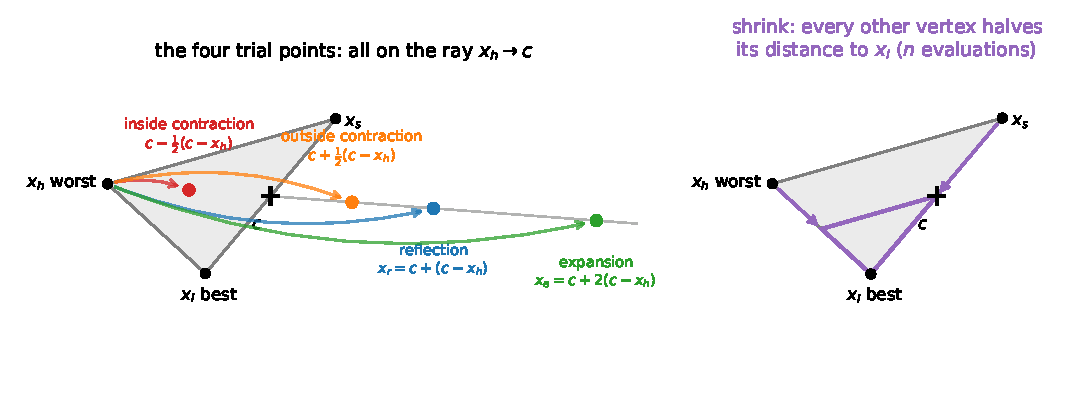
\includegraphics[width=\textwidth]{fig_moves}
\caption{One Nelder--Mead iteration, drawn for $n=2$ (a triangle).  All four
trial points lie on the ray from the worst vertex $\xh$ through the centroid
$c$ of the other $n$ vertices; only the multiple of $(c-\xh)$ differs.  Each
costs one objective evaluation, and at most two are ever tried in one
iteration.  Only if all of them fail does the method shrink (right), which
costs $n$ evaluations and is the one move that changes more than a single
vertex.}
\label{fig:moves}
\end{figure}

Write $\delta=c-\xh$.  The four candidates, all on one line
(Figure~\ref{fig:moves}), are
\begin{align}
  \text{reflection}         &\quad \xr=c+\alpha\,\delta, \\
  \text{expansion}          &\quad \xe=c+\gamma\,\delta, \\
  \text{outside contraction}&\quad \xc=c+\rho\,\delta, \\
  \text{inside contraction} &\quad \xc=c-\rho\,\delta,
\end{align}
and the decision is a short cascade:
\begin{enumerate}
\item Evaluate $\xr$.
\item If $q(\xr)<q(\xl)$ --- a new best --- try $\xe$ as well and keep
  whichever of the two is better.  \emph{(2 evaluations.)}
\item Else if $q(\xr)<q(\xs)$ --- an improvement, but not a new best ---
  accept $\xr$ in place of $\xh$.  \emph{(1 evaluation.)}
\item Else the ray overshot.  Contract: outside if $q(\xr)<q(\xh)$, inside
  otherwise, and accept the contracted point if it beats what it was compared
  against.  \emph{(2 evaluations.)}
\item If even the contraction fails, \textbf{shrink}: every vertex but the
  best moves halfway to the best,
  $x_i\leftarrow \xl+\sigma\,(x_i-\xl)$.  \emph{($n$ evaluations.)}
\end{enumerate}

So a typical iteration costs one or two evaluations regardless of $n$, and a
shrink costs $n$.  This is the first real difference from the one-variable
case: in 1-D a shrink is a single extra evaluation and nothing to worry
about, whereas at $n=9$ it costs nine, and a run that shrinks often is
spending most of its budget rebuilding the simplex rather than exploring.
Figure~\ref{fig:landscape} shows a measured move histogram.

\subsection{The coefficients depend on $n$}

With the textbook constants $(\alpha,\gamma,\rho,\sigma)=(1,2,\tfrac12,
\tfrac12)$ the simplex, in high dimension, tends to collapse into a
low-dimensional sliver and stall.  The adaptive choice of Gao and
Han\footnote{F.~Gao and L.~Han, \emph{Comput.\ Optim.\ Appl.} \textbf{51}
(2012) 259--277.  This is \texttt{adaptive=True} in
\texttt{scipy.optimize.minimize}, which the script passes.} scales them with
the dimension:
\begin{equation}
  \alpha=1,\qquad
  \gamma=1+\frac2n,\qquad
  \rho=\frac34-\frac1{2n},\qquad
  \sigma=1-\frac1n .
  \label{eq:adaptive}
\end{equation}
Expansion becomes timid and contraction and shrink become gentle as $n$ grows,
which is what keeps a ten-vertex simplex from degenerating
(Table~\ref{tab:adaptive}).  Two remarks:
\begin{itemize}
\item At $n=2$ the adaptive values coincide with the textbook ones, so the
  two-dimensional illustrations in this note are not a special case.
\item At $n=1$ the adaptive rule gives $\sigma=0$: a shrink collapses the
  segment onto its best point and the run stops at once.  That is degenerate,
  but harmless here --- the $D=1$ rung exists only to put the search in the
  right basin, and it is over in nine evaluations.
\end{itemize}

\begin{table}[htb]
\centering
\begin{tabular}{lrrrrr}
\toprule
$n$ (free variables) & 1 & 3 & 5 & 7 & 9 \\
\midrule
expansion   $\gamma$ & 3.000 & 1.667 & 1.400 & 1.286 & 1.222 \\
contraction $\rho$   & 0.250 & 0.583 & 0.650 & 0.679 & 0.694 \\
shrink      $\sigma$ & 0.000 & 0.667 & 0.800 & 0.857 & 0.889 \\
\bottomrule
\end{tabular}
\caption{The adaptive coefficients \eqref{eq:adaptive} at the five rungs of
the ladder.  Reflection is always $\alpha=1$.}
\label{tab:adaptive}
\end{table}

\subsection{Stopping}

The run stops when the simplex is small \emph{and} flat:
\begin{equation}
  \max_i\lVert x_i-x_0\rVert_\infty \le \mathtt{xatol}=10^{-3}\px
  \quad\text{and}\quad
  \max_i|q(x_i)-q(x_0)| \le \mathtt{fatol}=10^{-6}\ \text{nats}.
\end{equation}
Both are physical thanks to the normalisation \eqref{eq:units}: a thousandth
of a pixel, and a millionth of a nat against an entropy of $\approx4.8$.  A
budget \texttt{maxfev} caps each rung independently; in the verified run the
last two rungs hit the cap rather than the tolerances.

\subsection{What else changes when $n>1$}

\begin{description}
\item[No derivative, and none implied.] The method never estimates a gradient.
  It only ever compares values.  This is why it survives an objective built
  out of an FBP and a histogram, which is piecewise smooth at best: histogram
  binning makes $q$ a step function at the finest scale, and no finite
  difference of it means anything below the bin width.
\item[Cost grows only through the simplex.] Building the initial simplex costs
  $n+1$ evaluations, a shrink costs $n$, everything else costs $1$ or $2$.
  What really grows with $n$ is the \emph{number of iterations} needed, not
  the cost of one.
\item[It is not rotation invariant.] This is the property that bites here.
  Reflection and contraction are defined through the centroid of the current
  vertices, so the trajectory depends on the shape and orientation of the
  initial simplex.  Two runs from the same $x_0$ on the same objective, with
  the initial simplex built along different orthonormal axes, are different
  algorithms.  Section~\ref{sec:init} is about exactly this.
\item[Local, and with no guarantee.] Convergence to a stationary point is not
  proved in general for $n>1$; McKinnon's counterexample has it converge to a
  non-stationary point.  In practice it stalls in whichever basin its first
  simplex committed it to.
\end{description}

\section{Initialisation}
\label{sec:init}

This is the part that had to be got right, and the part that is different from
the one-variable picture.  There are three separate decisions.

\subsection{The starting point}

$x_0=0$: no correction, the raw sinogram.  There is no better guess available
without a reference, and the objective is well defined there --- indeed the
histogram range is measured at exactly this point, so $x_0$ is the reference
configuration of the whole score.  Its value, $q=4.80478$ nats at
$1.1083\px$ rms of identifiable error, is the number every later entropy is
judged against.

\subsection{The initial simplex, and why it is written out explicitly}

The script passes \texttt{initial\_simplex} rather than letting SciPy build
one:
\begin{equation}
  x_0,\quad x_0+h\,e_1,\quad\dots,\quad x_0+h\,e_n,
  \qquad h=1\px \text{ rms of shift}.
\end{equation}
This matters.  SciPy's default simplex perturbs each coordinate by $5\,\%$ of
its value, and \emph{a coordinate that is zero is perturbed by
$2.5\times10^{-4}$}.  Starting from $x_0=0$, the default simplex would
therefore have edges of a quarter of a thousandth of a pixel --- smaller than
\texttt{xatol}, so the run would report convergence almost immediately, at the
starting point, having learnt nothing.  A one-variable run started from a
nonzero guess never shows this, which is why it is easy to miss.

The edge length $h$ is the one number in the method that has to match the
problem.  The first simplex is the only global look Nelder--Mead ever takes:
everything afterwards is generated from it by reflection and contraction, so
the initial edge sets the scale on which the objective is first probed.  It
should be the size of the drift one expects to find --- here $1\px$ against a
true drift of $1.55\px$ rms, of which $1.11\px$ is identifiable.  Too small
and the simplex never leaves the local structure around $x_0$; too large and
the first reflections land in a region where the reconstruction is so blurred
that the entropy differences are noise.

\subsection{The ladder: each rung initialises the next}
\label{sec:ladder}

A single nine-dimensional descent from zero \emph{does not reliably work}, and
the reason is the rotation dependence above.  The columns of the free basis
come out of an SVD; their orientation is arbitrary, nothing in the problem
picks it.  Measured on this problem with six random orthogonal rotations of
that basis --- same subspace, same objective, same starting point, same budget
--- \textbf{two of the six stalled at entropy $4.8658$ instead of $4.8639$
and left the drift worse than no correction at all} ($1.6\px$ against
$1.1\px$).  A coin flip decided by a choice that carries no information.

Two things follow.  First, the failure is visible \emph{without the truth}:
the entropy reached is plainly higher, so a real scan can tell a bad run from
a good one.  Second, the cure is to never pose the nine-dimensional problem
cold.  The script fits coarse to fine:

\begin{enumerate}
\item $D=1$: one free variable.  Initial point $0$, initial simplex edge
  $1\px$.
\item For $D=2,\dots,5$: build the design matrix $P_D$ and the free basis
  $V_D$ for that degree, then \emph{initialise from the previous answer} by
  expressing it in the new basis,
  \begin{equation}
    a_D = \arg\min_a \lVert V_D\,a - \mathrm{vec}\,c_{D-1}\rVert ,
  \end{equation}
  padding $c_{D-1}$ with zeros up to degree $D$.  The simplex is rebuilt at
  full size, $a_D+1\px\cdot e_i$, around that point.
\end{enumerate}

Each rung is small enough that Nelder--Mead is reliable in it, and each starts
where the previous one finished, so no rung is ever far from its own minimum.
All six basis orientations then converge.  \texttt{maxfev} is a budget
\emph{per rung}, not for the whole run.

Rebuilding the simplex at full size on every rung is deliberate: the new
variables are genuinely unexplored, and a simplex inherited at the size the
previous rung had shrunk to would be far too small to find them.  The price is
the visible bump in entropy at the start of each rung in
Figure~\ref{fig:ladder} --- the new vertices are worse than the point they
were built around --- which costs a few tens of evaluations and buys the
reliability.

\section{What it actually does}

\subsection{On a two-dimensional slice of the real objective}

\begin{figure}[htb]
\centering
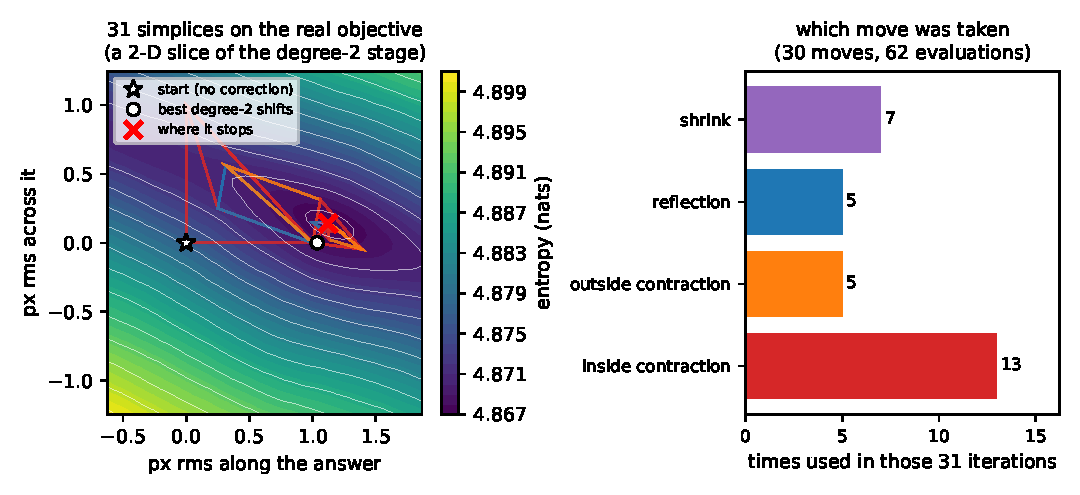
\includegraphics[width=\textwidth]{fig_landscape}
\caption{Left: the true objective --- entropy of the FBP --- on a plane
through the starting point and the best degree-2 drift, measured on a
$49\times49$ grid ($2401$ reconstructions).  The white star is $x_0$, the
white circle the best degree-2 point, the red cross where the simplex stops.
The $31$ triangles are the successive simplices, each coloured by the move
that produced it; the colours are the key of the right panel.  Right: how
often each move was used.  The run is dominated by inside contractions, with
seven shrinks --- the simplex spends most of its life pulling itself in around
the minimum.  The simplex shown is a hand-written Nelder--Mead that records
every move; its answer, $4.866962$ at $(1.1242,0.1412)$, is identical to
SciPy's.}
\label{fig:landscape}
\end{figure}

The plane of Figure~\ref{fig:landscape} is the degree-2 stage of the ladder,
which has three free variables, cut by the plane through $x_0$ and the best
degree-2 point.  The landscape is a smooth basin over a range of
$4.867$--$4.901$ nats, tilted, with the minimum offset from the true answer:
the white circle and the red cross do not coincide.  The offset is the
accuracy of the metric, not a failure of the search, and it is the reason the
last section reports the distance to the truth separately from the entropy.

\subsection{The full run}

\begin{figure}[htb]
\centering
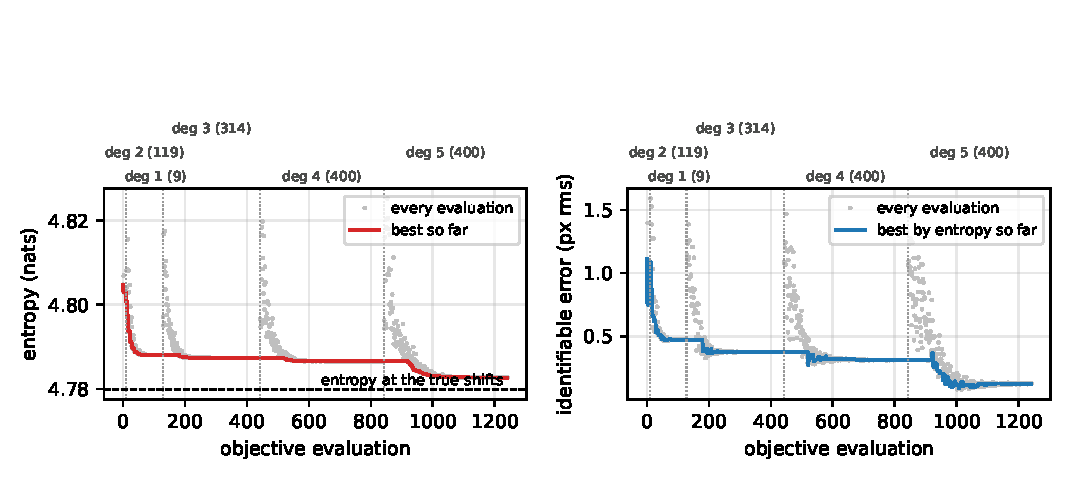
\includegraphics[width=\textwidth]{fig_ladder}
\caption{The verified run: \texttt{--nslice 16 --ntheta 192}, $1242$
evaluations, $6.5$~s on one A100.  Left, the objective the search sees;
right, the quantity it does not --- the rms distance to the true drift, after
the gauge \eqref{eq:gauge} is removed from both.  Grey dots are every
evaluation, including the trial points that get thrown away; the coloured line
is the best point so far.  Dotted lines are rung boundaries, labelled with
the degree and the evaluations it used.  Each rung starts with a burst of
worse values as the simplex is rebuilt at full size in the larger space, then
descends.  The two curves fall together, which is the whole claim of the
method: entropy is a usable stand-in for the alignment error.}
\label{fig:ladder}
\end{figure}

\begin{table}[htb]
\centering
\begin{tabular}{lrrrr}
\toprule
rung & free vars & evaluations & entropy (nats) & identifiable error \\
\midrule
start  & --- & ---  & 4.80478 & $1.1083\px$ \\
$D=1$  &  1  &    9 & 4.80293 & $0.7567\px$ \\
$D=2$  &  3  &  119 & 4.78802 & $0.4730\px$ \\
$D=3$  &  5  &  314 & 4.78734 & $0.3747\px$ \\
$D=4$  &  7  &  400 & 4.78654 & $0.3109\px$ \\
$D=5$  &  9  &  400 & 4.78269 & $0.1238\px$ \\
\bottomrule
\end{tabular}
\caption{The ladder, \texttt{--nslice 16 --ntheta 192}.  $88.8\,\%$ of the
identifiable drift is removed, against $90.4\,\%$ for the older script with
three restarts and twice the evaluations.  The recovered quintic coefficients
match the truth to a few thousandths of a pixel in the leading terms
($+2.0020/-1.5396$ against $+2.0/-1.5$ in $y$).}
\label{tab:ladder}
\end{table}

Table~\ref{tab:ladder} and Figure~\ref{fig:ladder} are the same run.  Three
numbers to read together at the end of it:
\begin{center}
\begin{tabular}{lr}
\toprule
entropy found by the search                      & $4.78269$ \\
entropy at the truth with the gauge removed      & $4.78324$ \\
entropy at the true shifts                       & $4.77979$ \\
\bottomrule
\end{tabular}
\end{center}
The search ends \emph{below} the point of its own space that is closest to the
truth --- so it has not failed to converge; the minimum of the metric is
simply displaced, by about a tenth of a pixel, which is the accuracy this kind
of autofocus has.  It ends above the entropy at the full true shifts because
those include the rigid part, which the search deliberately cannot reach and
which the fixed cylinder mask makes very slightly favourable.  No amount of
optimiser effort closes either gap: they are properties of the score, not of
Nelder--Mead.

\section{Practical summary}

\begin{itemize}
\item Normalise the search variables so one unit is one pixel rms of shift.
  Everything downstream --- the simplex edge, \texttt{xatol}, the plots ---
  then means something.
\item Project out the gauge before searching, or three of the dimensions are a
  flat valley.
\item Always pass \texttt{initial\_simplex} explicitly when starting from
  zero.  SciPy's default is $2.5\times10^{-4}$ there and the run converges
  immediately, at the starting point.
\item Set the edge to the drift you expect.  It is the only global look the
  method takes.
\item Use \texttt{adaptive=True} above a few dimensions.
\item Do not pose the full problem cold.  Climb a ladder of model complexity
  and initialise each rung from the previous answer; rebuild the simplex at
  full size on each rung.
\item Judge a run by the entropy it reaches, not by whether it reports
  success.  A bad orientation, a bad basin and an exhausted budget all look
  the same from the outside --- except in the value of the objective, which
  needs no ground truth.
\end{itemize}

\end{document}
